\section{Fixed-size LS-SVM}
As the number of data points increases working in the dual space becomes harder and harder, because the dimension of the unknown support vectors depends on the number of input data points $\alpha \in \mathcal{R}^N$. The primal problem is better suited for many input data points as the unknown primal weights vector length is determined by the dimension of the input data $\mathbf{w} \in \mathcal{R}^n$. In other words large data set problems should be solved in the primal space, while the dual space should be used if the input data is high dimensional. \footnote{Support Vector Machines: Methods and Applications, Suykens et al., page 174}
When SVMs are trained in the primal space, they are called fixed size svms. For the primal space case the kernel trick made it possible to train svms without explicitly knowing which non-linear function mapped to the feature space. When working in the primal space $\varphi(\mathbf{x})$ must be evaluated. This is only simple for linear classifiers, where $\varphi(\mathbf{x}) = \mathbf{x}$. In the non-linear case the Nystr\"{o}m method is required to approximate the nonlinear mapping $\varphi(\mathbf{x})$, the general idea is to choose a a fixed subsampled kernel matrix size $M$. Typically $M$ is a lot smaller then the true Kernel-matrix size $M \ll N$\footnote{Support Vector Machines: Methods and Applications, Suykens et al., page 175}  
This smaller kernel matrix is then approximated using a subset of the input data. The computed eigenvalues and eigenvector found from this set are then used as an approximation to the true large version of the matrix. 
Instead of choosing these support vectors randomly the entropy function,\footnote{Support Vector Machines: Methods and Applications, Suykens et al., page 181} 
\begin{align}
H_r = = - \log\int p(\mathbf{x})^2 d\mathbf{x} \\
\int p(\mathbf{x})^2 d\mathbf{x} = \frac{1}{N^2} \mathbf{1}^T \Omega \mathbf{1}
\end{align}
is used. Starting from a random fixed size pool of support vectors a selected vector is replace with a value from the training set. If the entropy increases the datum is kept in the support vector set. If the entropy function does not increase the new value is rejected and the old one is kept in the set. This procedure is repeated until the entropy function does int increase sufficiently anymore or a maximum number of iteration is reached. The reduced kernel matrix can be determined from the fixed set. After estimating its eigenfunction $\mathbf{w}$ and $b$ are determined.
\begin{figure}
\centering
% This file was created by matlab2tikz.
% Minimal pgfplots version: 1.3
%
%The latest updates can be retrieved from
%  http://www.mathworks.com/matlabcentral/fileexchange/22022-matlab2tikz
%where you can also make suggestions and rate matlab2tikz.
%
\documentclass[tikz]{standalone}
\usepackage{pgfplots}
\usepackage{grffile}
\pgfplotsset{compat=newest}
\usetikzlibrary{plotmarks}
\usepackage{amsmath}

\begin{document}
\definecolor{mycolor1}{rgb}{0.00000,0.44700,0.74100}%
%
\begin{tikzpicture}

\begin{axis}[%
width=2.5in,
height=1.5in,
scale only axis,
xmin=0,
xmax=100,
ymin=0,
ymax=2.5,
xlabel={iterations},
ylabel={$H_r$}
]
\addplot [color=mycolor1,solid,forget plot]
  table[row sep=crcr]{%
1	0.19845093872309\\
2	0.258665384669612\\
3	0.479609523381547\\
4	0.723809571263707\\
5	0.723809571263707\\
6	0.987639124316571\\
7	0.987639124316571\\
8	0.987639124316571\\
9	0.987639124316571\\
10	1.27994165616571\\
11	1.52701781174902\\
12	1.70972641923852\\
13	1.72165581443517\\
14	1.72165581443517\\
15	1.72165581443517\\
16	1.72165581443517\\
17	1.74755871381816\\
18	1.85718279280368\\
19	2.07286545623056\\
20	2.07286545623056\\
21	2.07286545623056\\
22	2.07286545623056\\
23	2.07286545623056\\
24	2.07286545623056\\
25	2.09416283678939\\
26	2.09416283678939\\
27	2.09416283678939\\
28	2.15896702947032\\
29	2.15896702947032\\
30	2.15896702947032\\
31	2.15896702947032\\
32	2.15896702947032\\
33	2.15896702947032\\
34	2.15896702947032\\
35	2.15896702947032\\
36	2.15896702947032\\
37	2.2167326293599\\
38	2.21674738661427\\
39	2.21674738661427\\
40	2.21879211543706\\
41	2.21879211543706\\
42	2.21879211543706\\
43	2.21879211543706\\
44	2.21879211543706\\
45	2.21879211543706\\
46	2.21879211543706\\
47	2.21879211543706\\
48	2.21879211543706\\
49	2.27375160458011\\
50	2.27375160458011\\
51	2.27375160458011\\
52	2.27942454075771\\
53	2.27942454075771\\
54	2.27942454075771\\
55	2.27942454075771\\
56	2.29430719618184\\
57	2.29430719618184\\
58	2.29430719618184\\
59	2.29430719618184\\
60	2.29430719618184\\
61	2.29430719618184\\
62	2.29430719618184\\
63	2.29430719618184\\
64	2.29430719618184\\
65	2.29430719618184\\
66	2.29430719618184\\
67	2.29430719618184\\
68	2.29430719618184\\
69	2.29430719618184\\
70	2.29430719618184\\
71	2.29430719618184\\
72	2.29430719618184\\
73	2.29430719618184\\
74	2.29430719618184\\
75	2.29430719618184\\
76	2.29430719618184\\
77	2.29430719618184\\
78	2.29430719618184\\
79	2.29430719618184\\
80	2.29430719618184\\
81	2.29430719618184\\
82	2.29430719618184\\
83	2.29430719618184\\
84	2.29430719618184\\
85	2.29430719618184\\
86	2.29430719618184\\
87	2.29430719618184\\
88	2.29430719618184\\
89	2.29430719618184\\
90	2.29430719618184\\
91	2.29430719618184\\
92	2.29430719618184\\
93	2.29430719618184\\
94	2.29430719618184\\
95	2.29430719618184\\
96	2.29430719618184\\
97	2.29430719618184\\
98	2.29430719618184\\
99	2.29430719618184\\
100	2.29430719618184\\
};
\end{axis}
\end{tikzpicture}%
\end{document}
\caption{The value of the entropy function for an optimization process of a subset of 10 values drawn from the normal distribution $\mathcal{N}(0,2^2)$}
\label{fig:normalEntropy}
\end{figure}
Figure~\ref{fig:normalEntropy} shows the entropy function over hundred iterations of a ten vector subset from a normally distributed data-set. 
\begin{figure}
% This file was created by matlab2tikz.
% Minimal pgfplots version: 1.3
%
%The latest updates can be retrieved from
%  http://www.mathworks.com/matlabcentral/fileexchange/22022-matlab2tikz
%where you can also make suggestions and rate matlab2tikz.
%
\documentclass[tikz]{standalone}
\usepackage{pgfplots}
\usepackage{grffile}
\pgfplotsset{compat=newest}
\usetikzlibrary{plotmarks}
\usepackage{amsmath}

\begin{document}
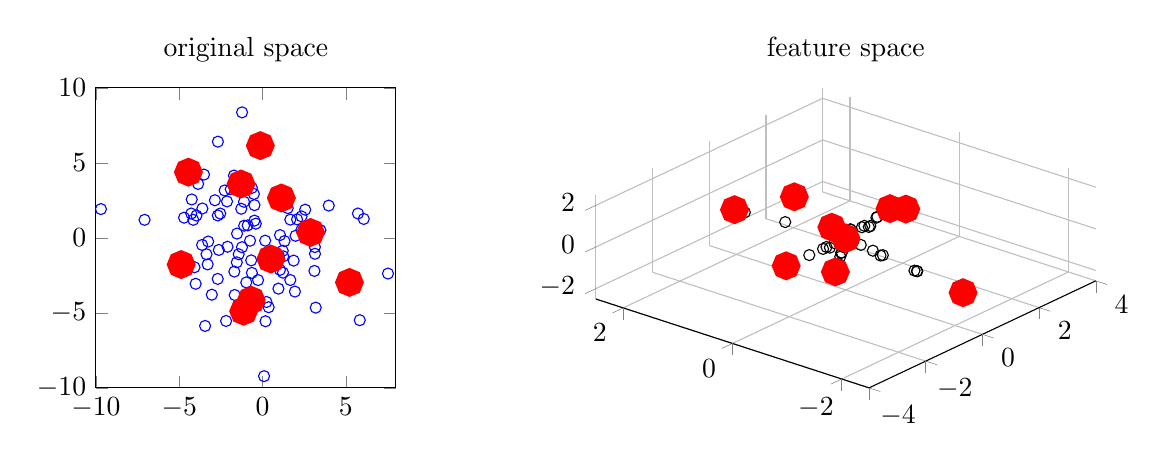
\begin{tikzpicture}

\begin{axis}[%
width=1.5in,
height=1.5in,
at={(0in,0in)},
scale only axis,
xmin=-10,
xmax=8,
ymin=-10,
ymax=10,
title={original space}
]
\addplot [color=blue,only marks,mark=o,mark options={solid},forget plot]
  table[row sep=crcr]{%
-1.13447116976927	-4.89162867824175\\
-4.44802833317701	4.38003955542794\\
-0.131455756074884	6.1501281988136\\
2.88247563504634	0.361501799098167\\
5.21473479784002	-2.96970481266356\\
-1.2906187272783	3.59331442294463\\
-4.88196820940934	-1.77796865450776\\
0.499042477380197	-1.40942808967336\\
1.12879773135216	2.65913213121808\\
-0.680851394118698	-4.15565940333251\\
-3.44673686885637	-5.87026186269576\\
6.07299779863161	1.26205110060375\\
-7.07857053287547	1.20221399444089\\
-1.52991613739982	0.285426473592506\\
-3.9648767724303	1.49005317490959\\
-1.90838474898012	3.24672178848209\\
0.95355425717909	2.91134336506372\\
0.414143923348578	-1.70570871116882\\
-2.13220522443368	2.42991621995562\\
2.33101058015936	0.519742115496264\\
1.86718177251604	-1.51662770554614\\
1.94214265354814	-3.57991737267061\\
-1.27689504498105	1.94091281664345\\
3.14574228160932	-1.06086779789802\\
1.98212125910152	0.139303580063469\\
7.52631741955532	-2.37884250660542\\
3.19037891712307	-4.65154342433868\\
3.47076495998218	0.514759065805883\\
0.158936481976839	-0.186417374413085\\
-3.86515800882087	3.5970836318759\\
-1.1136637424929	2.40511221098183\\
-2.27337574949646	3.15991373744864\\
-1.69190675108228	-2.24663025762948\\
1.66541568000554	-2.80897949134806\\
-1.6703341918511	-3.80726031860547\\
-2.68533940644731	1.4939418691402\\
-1.22798316490221	8.36724338293177\\
-0.482660300215329	2.18271611074717\\
1.22800329136637	-2.31919230645671\\
-2.85790799135993	2.50990126342846\\
0.951952416973836	-3.38499093025081\\
0.234060242934233	-4.27341027424914\\
3.97315634748067	2.15232694652207\\
-0.639511459264758	-2.33371656055619\\
-0.403435933666279	0.947957642125813\\
-3.51406745376089	4.21960541423037\\
-4.15578804958572	1.20337390719559\\
0.931524955801496	2.78898085325897\\
-0.748467193421817	-4.81740661386225\\
1.51123216721198	1.98460873237023\\
-2.67798421043111	6.41550676148554\\
5.72553699107467	1.62341824025139\\
0.36669210151466	-4.62263154557365\\
3.1410998006938	-0.609428384465502\\
-0.680760597971811	-1.49989566533803\\
-0.487505824645485	1.14907173834249\\
2.07015569357342	1.23610613433525\\
1.66727031423631	1.21647765154932\\
-3.36076500446523	-1.09134225264305\\
-4.59807904178853	-1.79781612012584\\
-3.29360330862201	-1.7687669742541\\
-4.24731996470382	2.56062250219344\\
0.178711765698137	-5.55902421425879\\
-1.23375277659666	-0.621909478942874\\
-1.10403219912287	0.811134608069748\\
-4.08288938818108	-1.95831303617678\\
2.33870228620492	1.43168185502302\\
1.31823333466114	-0.213958950082362\\
-0.268867451223629	-2.81490386480645\\
3.06354035404255	0.484090603951908\\
-2.62193839508671	-0.804548645740165\\
1.24410087914288	-1.22961794327023\\
1.04532359985684	-2.13396813157842\\
1.04776324999114	0.184336450752292\\
-2.18774180288851	-5.53838770829578\\
0.980520746288974	-1.19499935843439\\
-1.54464489877943	-1.63064436483716\\
-2.68933845150746	-2.73569551286598\\
-3.60980455924505	1.95809577298572\\
3.11344691845572	-2.20281377577274\\
-2.53783263700835	1.62189926944334\\
-0.518741532777503	2.92752265374548\\
-3.6259561642206	-0.470611244181153\\
-0.891380399986213	0.833397965170124\\
-9.69611338782002	1.91855190933262\\
-3.26087768838399	-0.242934045181829\\
-4.27930847843917	1.62261043129181\\
-3.04335230311596	-3.78769453388387\\
-0.639801564922074	3.33127152201048\\
-0.976043341081473	-2.96868803720509\\
5.83319337589885	-5.48650780261153\\
-1.71531965504837	4.15349553406279\\
-0.750096834105132	-0.188180382123768\\
-4.70794641102209	1.34676336005751\\
-1.4321479910822	-1.08977541740301\\
-4.01392996068678	-3.06175017939306\\
0.0908970713645493	-9.2189656178612\\
2.55926030255573	1.87883699309742\\
1.21276039532808	-0.860053599633674\\
-2.10186064025462	-0.592028720552758\\
};
\addplot [color=red,line width=6.0pt,only marks,mark=o,mark options={solid},forget plot]
  table[row sep=crcr]{%
-1.13447116976927	-4.89162867824175\\
-4.44802833317701	4.38003955542794\\
-0.131455756074884	6.1501281988136\\
2.88247563504634	0.361501799098167\\
5.21473479784002	-2.96970481266356\\
-1.2906187272783	3.59331442294463\\
-4.88196820940934	-1.77796865450776\\
0.499042477380197	-1.40942808967336\\
1.12879773135216	2.65913213121808\\
-0.680851394118698	-4.15565940333251\\
};
\end{axis}

\begin{axis}[%
width=2.5in,
height=1.5in,
at={(2.5in,0in)},
scale only axis,
xmin=-4,
xmax=4,
tick align=outside,
ymin=-2.5,
ymax=2.5,
zmin=-2.5,
zmax=2.5,
view={-50.3}{53.2},
title={feature space},
axis x line*=bottom,
axis y line*=left,
axis z line*=left,
grid = major
]
\addplot3 [color=black,only marks,mark=o,mark options={solid}]
 table[row sep=crcr] {%
2.1076856997482	-0.00373250713567108	0.0316398820726253\\
2.597319812798e-09	0.256067533490578	0.293306421262291\\
1.40125522750489e-09	0.942727533777028	1.16976603556955\\
-0.00110940035224929	-0.809150351923737	2.09772659291241\\
9.33997723241364e-08	0.0049178557802949	-0.0388404409746971\\
-3.5039195307987e-07	-2.14496077028076	-0.801620475153491\\
9.88136093124369e-06	-1.94316008422322e-06	4.92465674088906e-05\\
0.0627391064503034	0.224311402126535	-1.86761482009978\\
5.51492883726411e-06	2.03784190339991	-0.383943600215639\\
-2.10849655158651	-0.00171569180531476	0.0155499887903112\\
0.00722090879734848	-6.84909891808436e-06	5.6972941703479e-05\\
-1.88653434321038e-08	-1.36528776777426e-05	3.53787082662861e-05\\
1.10191083399309e-11	1.04085490852971e-08	1.19779212159235e-08\\
5.83117791779227e-05	0.000177185811326557	-0.00173637028307621\\
9.51790361950651e-11	2.76665703743076e-05	4.72638471190063e-05\\
-2.15938431771046e-07	-1.30013290645637	-0.485233124524682\\
5.21428989220289e-06	1.84814673147073	-0.352146031307017\\
0.0545607311844174	0.204068322693835	-1.69859133772935\\
-4.53044249469533e-08	-0.273186217399918	-0.101966498381235\\
-0.000751610367922941	-0.577443460937592	1.50714099681312\\
0.0096045028364302	0.0256472374581142	-0.26209882221488\\
-0.00282915626329713	0.000251565637168164	-0.00209312504566487\\
2.33015540053735e-08	-0.136253949329163	-0.0529510291186149\\
-8.72056097513135e-05	-0.0997183390439414	0.257358614002137\\
0.000163736627144279	-0.338633652338516	0.868689282435268\\
3.1509869687558e-10	1.65784927758512e-05	-0.000130933340807213\\
-9.41343612679739e-07	4.83045075522378e-06	-3.8151437074705e-05\\
-0.000772880688308526	-0.559415899788871	1.44982279219543\\
0.0126272252164957	0.0446792425623654	-0.371955106800821\\
5.32662085659417e-10	0.0959396465627591	0.112068934045808\\
-4.66885843919275e-08	-0.494745507457085	-0.191682373819238\\
-1.12680579967151e-07	-0.677060284554494	-0.252311621878907\\
-0.0347168532732219	0.000913888656219164	-0.00759415047607578\\
-0.000346099625904672	0.0081126415969537	-0.0675655590713782\\
-0.405339566052626	-0.000851335867348045	0.00750570671341563\\
-7.50079603355697e-11	-0.00373881093440734	-0.00139345703432416\\
3.37099928355055e-12	0.00207853505017654	0.00257756757749403\\
3.77135686436239e-07	-0.0316973622522322	-0.079828515929661\\
0.012680484311427	0.057617507018841	-0.479772747464829\\
-9.46582857437776e-09	-0.0563215621200004	-0.0205433762215814\\
-0.147382462977547	0.00368599342697803	-0.0306289926573963\\
-1.29023360835199	-0.000323190243925588	0.00323578531431611\\
-1.37804852854084e-05	-0.00949025163232485	0.0257548231345524\\
-0.132738297365456	0.0261234564371379	-0.217377263100127\\
0.000108146460551933	0.0099133202218642	-0.00545656105537642\\
-6.58826757930213e-10	0.0939956420480058	0.115634167746103\\
8.04472951132636e-10	7.81255338785493e-06	1.04437444559342e-05\\
5.39372856874961e-06	1.92179418913461	-0.365549682593148\\
0.858161998359719	-0.0031909527384649	0.0273548887346193\\
-8.85453423205802e-06	1.10959851269971	-0.187260963308871\\
-1.4136451911496e-11	0.00141061921288642	0.00182688746586623\\
-7.02679872253241e-08	-5.08527531265495e-05	0.000131776580429179\\
-0.683546074998798	-0.000351019000891347	0.00326346717152259\\
-0.000376626377305261	-0.294904204829803	0.763559441584148\\
0.0121689597672826	0.0553373739383258	-0.460568368695276\\
3.43617316095874e-05	0.0125573864010893	-0.00494637322683848\\
-0.00026392278264742	-0.0837184926503207	0.483701469252029\\
-0.000106111002982722	0.101560083997061	0.194402325378792\\
3.8971215557985e-07	-5.12060302705862e-08	2.46675351020467e-06\\
9.1111242679273e-06	-1.79199376074095e-06	4.54154698355889e-05\\
-1.15500713792973e-05	-4.61357167444152e-08	3.04181344792059e-06\\
7.17886590687007e-11	0.0088627276913464	0.0102413178798884\\
0.190336650908329	-0.000425865303280913	0.00362622820430037\\
0.0016786626423368	0.00599438192534403	-0.049889928213473\\
3.49661429733335e-05	-0.000319455332992285	-0.00145496018404618\\
4.87282637890522e-06	-9.93273417852713e-07	2.51733999322191e-05\\
-0.000263845510140149	-0.0870053882302502	0.476928749638208\\
0.00767603736392872	-0.0223414904111555	-0.0983633891022214\\
-0.529767184809212	0.0172425634993477	-0.143328915287328\\
-0.00106410110952997	-0.771427930752271	1.99998686361974\\
1.40204985829514e-06	9.15469922940685e-06	-7.61285099956412e-05\\
0.0351348133242197	0.120331413688829	-1.02670135336882\\
0.0243717150226679	0.0984582889220889	-0.819773811190419\\
0.00365456847929578	-0.0095539095527762	-0.0396483294352444\\
0.807996492395376	-0.000812649602544457	0.00677566333658522\\
0.0478783463141046	0.168067629312756	-1.40985989160519\\
-0.00222684941072671	0.00328037839646451	-0.0273013192258667\\
-0.00602013481338646	-1.650561557507e-06	1.68491317046502e-05\\
-1.08335812868386e-10	-0.000324008608473091	0.000156689614855525\\
3.47261095974928e-05	-0.000908265531096647	0.00144126326597458\\
-9.05712625719493e-10	-0.00929708184527298	-0.00346797021869688\\
2.2975988832504e-07	-0.634032265020724	-0.307202637308177\\
3.69548230899708e-07	-6.94468299182676e-08	1.80884071861095e-06\\
5.98355558228329e-05	0.000540378408513497	-0.00233276534876884\\
9.95892968289794e-22	6.54002113781361e-16	7.49009431498825e-16\\
7.82639860762829e-08	1.04955702184598e-08	-1.69568011704629e-08\\
6.55961121419843e-11	0.000118318679878417	0.000140011704584959\\
0.01778134235418	-2.88663297226859e-05	0.000244236016718243\\
-5.73591605045715e-08	-1.25569302848408	-0.500366672685541\\
-0.799761535173201	0.00215577184212038	-0.0176548775553227\\
1.13140558673119e-10	5.95273292775121e-06	-4.70133934166737e-05\\
-2.177968939054e-07	-1.30866901520982	-0.487127957126098\\
0.00299024354561982	0.0106256801560032	-0.0883051855439449\\
5.51338452681787e-10	2.40522127455713e-05	2.76393390023662e-05\\
0.00118464239207372	0.00486416605423225	-0.0404840415210459\\
1.80499487990288e-05	-2.08849497685828e-07	4.73938677425436e-06\\
6.5587973937006e-09	-6.15114409250038e-12	5.11432621729117e-11\\
-0.000100383726058092	0.070485143488344	0.162093433646569\\
0.0280927632127055	0.0885219952307504	-0.80092334543207\\
3.58148102765191e-05	0.000132726325317952	-0.00110489401963831\\
};
 \addplot3 [color=red,line width=6.0pt,only marks,mark=o,mark options={solid}]
 table[row sep=crcr] {%
2.1076856997482	-0.00373250713567108	0.0316398820726253\\
2.597319812798e-09	0.256067533490578	0.293306421262291\\
1.40125522750489e-09	0.942727533777028	1.16976603556955\\
-0.00110940035224929	-0.809150351923737	2.09772659291241\\
9.33997723241364e-08	0.0049178557802949	-0.0388404409746971\\
-3.5039195307987e-07	-2.14496077028076	-0.801620475153491\\
9.88136093124369e-06	-1.94316008422322e-06	4.92465674088906e-05\\
0.0627391064503034	0.224311402126535	-1.86761482009978\\
5.51492883726411e-06	2.03784190339991	-0.383943600215639\\
-2.10849655158651	-0.00171569180531476	0.0155499887903112\\
};
 \end{axis}
\end{tikzpicture}%
\end{document}
\caption{Feature space reconstruction}
\label{fig:featureReconstr}
\end{figure}
Given this optimized subset the nonlinear mapping can be approximated as shown in figure~\ref{fig:featureReconstr} using the Nystr\"{o}m method, if alongside the selected inputs a kernel function and its parameters are chosen. 

\subsection{Sparsity and the $l_0$-norm}
\begin{figure}
\centering
% This file was created by matlab2tikz.
% Minimal pgfplots version: 1.3
%
%The latest updates can be retrieved from
%  http://www.mathworks.com/matlabcentral/fileexchange/22022-matlab2tikz
%where you can also make suggestions and rate matlab2tikz.
%
\documentclass[tikz]{standalone}
\usepackage{pgfplots}
\usepackage{grffile}
\pgfplotsset{compat=newest}
\usetikzlibrary{plotmarks}
\usepackage{amsmath}

\begin{document}
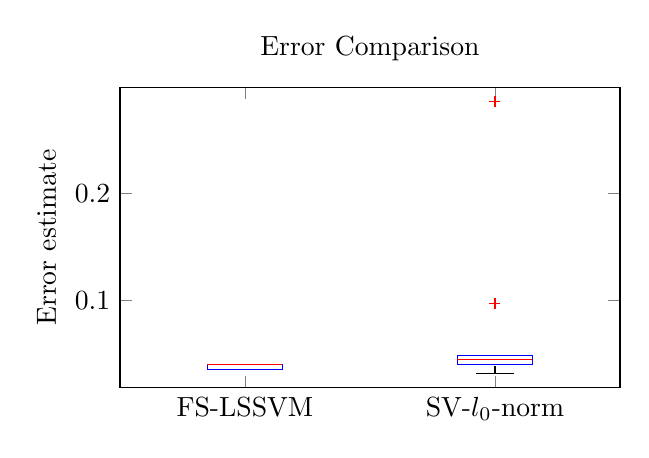
\begin{tikzpicture}

\begin{axis}[%
width=2.5in,
height=1.5in,
scale only axis,
unbounded coords=jump,
xmin=0.5,
xmax=2.5,
xtick={1,2},
xticklabels={{FS-LSSVM},{SV-$l_0$-norm}},
ymin=0.0180616740088106,
ymax=0.299118942731278,
ylabel={Error estimate},
title={Error Comparison}
]
\addplot [color=black,dashed,forget plot]
  table[row sep=crcr]{%
1	0.039647577092511\\
1	0.039647577092511\\
};
\addplot [color=black,dashed,forget plot]
  table[row sep=crcr]{%
2	0.0484581497797357\\
2	0.0484581497797357\\
};
\addplot [color=black,dashed,forget plot]
  table[row sep=crcr]{%
1	0.0352422907488987\\
1	0.0352422907488987\\
};
\addplot [color=black,dashed,forget plot]
  table[row sep=crcr]{%
2	0.0308370044052863\\
2	0.039647577092511\\
};
\addplot [color=black,solid,forget plot]
  table[row sep=crcr]{%
0.925	0.039647577092511\\
1.075	0.039647577092511\\
};
\addplot [color=black,solid,forget plot]
  table[row sep=crcr]{%
1.925	0.0484581497797357\\
2.075	0.0484581497797357\\
};
\addplot [color=black,solid,forget plot]
  table[row sep=crcr]{%
0.925	0.0352422907488987\\
1.075	0.0352422907488987\\
};
\addplot [color=black,solid,forget plot]
  table[row sep=crcr]{%
1.925	0.0308370044052863\\
2.075	0.0308370044052863\\
};
\addplot [color=blue,solid,forget plot]
  table[row sep=crcr]{%
0.85	0.0352422907488987\\
0.85	0.039647577092511\\
1.15	0.039647577092511\\
1.15	0.0352422907488987\\
0.85	0.0352422907488987\\
};
\addplot [color=blue,solid,forget plot]
  table[row sep=crcr]{%
1.85	0.039647577092511\\
1.85	0.0484581497797357\\
2.15	0.0484581497797357\\
2.15	0.039647577092511\\
1.85	0.039647577092511\\
};
\addplot [color=red,solid,forget plot]
  table[row sep=crcr]{%
0.85	0.039647577092511\\
1.15	0.039647577092511\\
};
\addplot [color=red,solid,forget plot]
  table[row sep=crcr]{%
1.85	0.0440528634361234\\
2.15	0.0440528634361234\\
};
\addplot [color=black,only marks,mark=+,mark options={solid,draw=red},forget plot]
  table[row sep=crcr]{%
nan	nan\\
};
\addplot [color=black,only marks,mark=+,mark options={solid,draw=red},forget plot]
  table[row sep=crcr]{%
2	0.0969162995594714\\
2	0.286343612334802\\
};
\end{axis}
\end{tikzpicture}%
\end{document}
% This file was created by matlab2tikz.
% Minimal pgfplots version: 1.3
%
%The latest updates can be retrieved from
%  http://www.mathworks.com/matlabcentral/fileexchange/22022-matlab2tikz
%where you can also make suggestions and rate matlab2tikz.
%
\documentclass[tikz]{standalone}
\usepackage{pgfplots}
\usepackage{grffile}
\pgfplotsset{compat=newest}
\usetikzlibrary{plotmarks}
\usepackage{amsmath}

\begin{document}
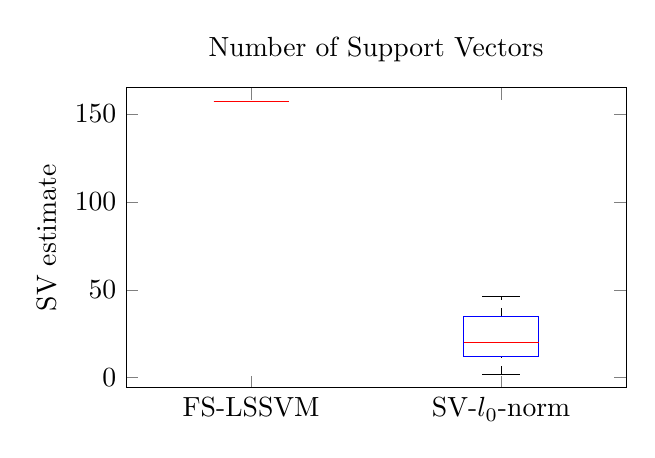
\begin{tikzpicture}

\begin{axis}[%
width=2.5in,
height=1.5in,
scale only axis,
unbounded coords=jump,
xmin=0.5,
xmax=2.5,
xtick={1,2},
xticklabels={{FS-LSSVM},{SV-$l_0$-norm}},
ymin=-5.75,
ymax=164.75,
ylabel={SV estimate},
title={Number of Support Vectors}
]
\addplot [color=black,dashed,forget plot]
  table[row sep=crcr]{%
1	157\\
1	157\\
};
\addplot [color=black,dashed,forget plot]
  table[row sep=crcr]{%
2	35\\
2	46\\
};
\addplot [color=black,dashed,forget plot]
  table[row sep=crcr]{%
1	157\\
1	157\\
};
\addplot [color=black,dashed,forget plot]
  table[row sep=crcr]{%
2	2\\
2	12\\
};
\addplot [color=black,solid,forget plot]
  table[row sep=crcr]{%
0.925	157\\
1.075	157\\
};
\addplot [color=black,solid,forget plot]
  table[row sep=crcr]{%
1.925	46\\
2.075	46\\
};
\addplot [color=black,solid,forget plot]
  table[row sep=crcr]{%
0.925	157\\
1.075	157\\
};
\addplot [color=black,solid,forget plot]
  table[row sep=crcr]{%
1.925	2\\
2.075	2\\
};
\addplot [color=blue,solid,forget plot]
  table[row sep=crcr]{%
0.85	157\\
0.85	157\\
1.15	157\\
1.15	157\\
0.85	157\\
};
\addplot [color=blue,solid,forget plot]
  table[row sep=crcr]{%
1.85	12\\
1.85	35\\
2.15	35\\
2.15	12\\
1.85	12\\
};
\addplot [color=red,solid,forget plot]
  table[row sep=crcr]{%
0.85	157\\
1.15	157\\
};
\addplot [color=red,solid,forget plot]
  table[row sep=crcr]{%
1.85	20\\
2.15	20\\
};
\addplot [color=black,only marks,mark=+,mark options={solid,draw=red},forget plot]
  table[row sep=crcr]{%
nan	nan\\
};
\addplot [color=black,only marks,mark=+,mark options={solid,draw=red},forget plot]
  table[row sep=crcr]{%
nan	nan\\
};
\end{axis}
\end{tikzpicture}%
\end{document}
% This file was created by matlab2tikz.
% Minimal pgfplots version: 1.3
%
%The latest updates can be retrieved from
%  http://www.mathworks.com/matlabcentral/fileexchange/22022-matlab2tikz
%where you can also make suggestions and rate matlab2tikz.
%
\documentclass[tikz]{standalone}
\usepackage{pgfplots}
\usepackage{grffile}
\pgfplotsset{compat=newest}
\usetikzlibrary{plotmarks}
\usepackage{amsmath}

\begin{document}
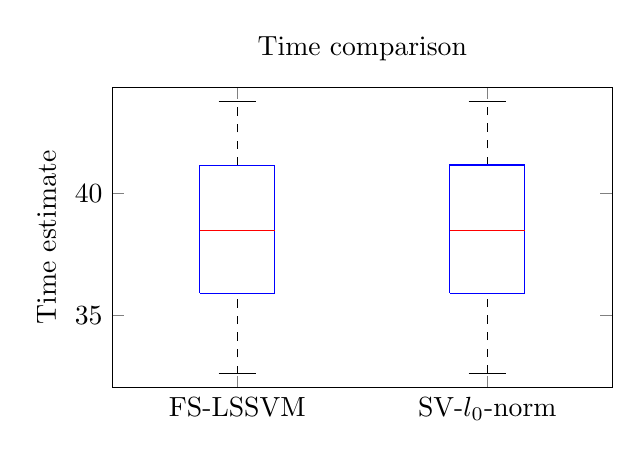
\begin{tikzpicture}

\begin{axis}[%
width=2.5in,
height=1.5in,
scale only axis,
unbounded coords=jump,
xmin=0.5,
xmax=2.5,
xtick={1,2},
xticklabels={{FS-LSSVM},{SV-$l_0$-norm}},
ymin=32.03,
ymax=44.35,
ylabel={Time estimate},
title={Time comparison}
]
\addplot [color=black,dashed,forget plot]
  table[row sep=crcr]{%
1	41.15\\
1	43.77\\
};
\addplot [color=black,dashed,forget plot]
  table[row sep=crcr]{%
2	41.17\\
2	43.79\\
};
\addplot [color=black,dashed,forget plot]
  table[row sep=crcr]{%
1	32.59\\
1	35.91\\
};
\addplot [color=black,dashed,forget plot]
  table[row sep=crcr]{%
2	32.61\\
2	35.91\\
};
\addplot [color=black,solid,forget plot]
  table[row sep=crcr]{%
0.925	43.77\\
1.075	43.77\\
};
\addplot [color=black,solid,forget plot]
  table[row sep=crcr]{%
1.925	43.79\\
2.075	43.79\\
};
\addplot [color=black,solid,forget plot]
  table[row sep=crcr]{%
0.925	32.59\\
1.075	32.59\\
};
\addplot [color=black,solid,forget plot]
  table[row sep=crcr]{%
1.925	32.61\\
2.075	32.61\\
};
\addplot [color=blue,solid,forget plot]
  table[row sep=crcr]{%
0.85	35.91\\
0.85	41.15\\
1.15	41.15\\
1.15	35.91\\
0.85	35.91\\
};
\addplot [color=blue,solid,forget plot]
  table[row sep=crcr]{%
1.85	35.91\\
1.85	41.17\\
2.15	41.17\\
2.15	35.91\\
1.85	35.91\\
};
\addplot [color=red,solid,forget plot]
  table[row sep=crcr]{%
0.85	38.47\\
1.15	38.47\\
};
\addplot [color=red,solid,forget plot]
  table[row sep=crcr]{%
1.85	38.485\\
2.15	38.485\\
};
\addplot [color=black,only marks,mark=+,mark options={solid,draw=red},forget plot]
  table[row sep=crcr]{%
nan	nan\\
};
\addplot [color=black,only marks,mark=+,mark options={solid,draw=red},forget plot]
  table[row sep=crcr]{%
nan	nan\\
};
\end{axis}
\end{tikzpicture}%
\end{document}
\caption{Classical fixed size svm and $l_0$ reduced version comparison for classification on the Wisconsin breast cancer dataset.}
\label{fig:brl0}
\end{figure}
Sparsity is a desirable property of trained support vector machines. In the dual space an ls-svm classifier is sparse if many support vectors are zero. \footnote{Support Vector Machines: Methods and Applications, Suykens et al., page 33} When evaluating the classifier only the non-zero vectors have to be taken into account, making the computation more efficient. For fixed size ls-svms the primal problem is considered, the notion of sparsity translates into a smaller representation of the basis given by:
\begin{equation}
\mathbf{w} = \sum\limits_{N}^{k = 1} \alpha_k \varphi(\mathbf{x}_k)
\end{equation}
A good method of determining suitable subset of the input space $\{\varphi(\mathbf{x}_k)\}_{k = 1}^N$, could for example be the entropy selection method discussed earlier. The determined subset could then serve as a way to approximate a sparse $\mathbf{w}$. This goal is formulated using the $l_0$ norm
\begin{equation}
\min\limits_{\mathbf{w}} \| \mathbf{w} \|_0 = \|w_1 \|^0 + \|w_2 \|^0 + \dots +\|w_N \|^0 
\end{equation}
which is equivalent to minimizing the count of non-zero elements in the vector.\footnote{David Wipf and Bhaskar Rao, $l_0$-norm Minimization for Basis Selection}
A first experiment using this method of producing sparsity is use for classification of the comparatively small Wisconsin data set. Results from running \texttt{fslssvm\_script} are shown in figure~\ref{fig:brl0}. The error comparison shows a slightly elevated median for the sparse version, probably due to the random nature of the input set reduction process bad outliers in terms of error exist. The figure also reveals, that the $l_0$ norm minimization process significatly reduced the number of support vectors, while it does not lead to a significant increase in training time.


